\section{Background, specification and related studies}

\subsection{Background and specification}

When there are too many bursts enter network, the performance of network will drop quickly. This phenomenon is known as congestion. 

\begin{figure}[!htb]
  \begin{minipage}[t]{0.5\linewidth} 
    \centering 
    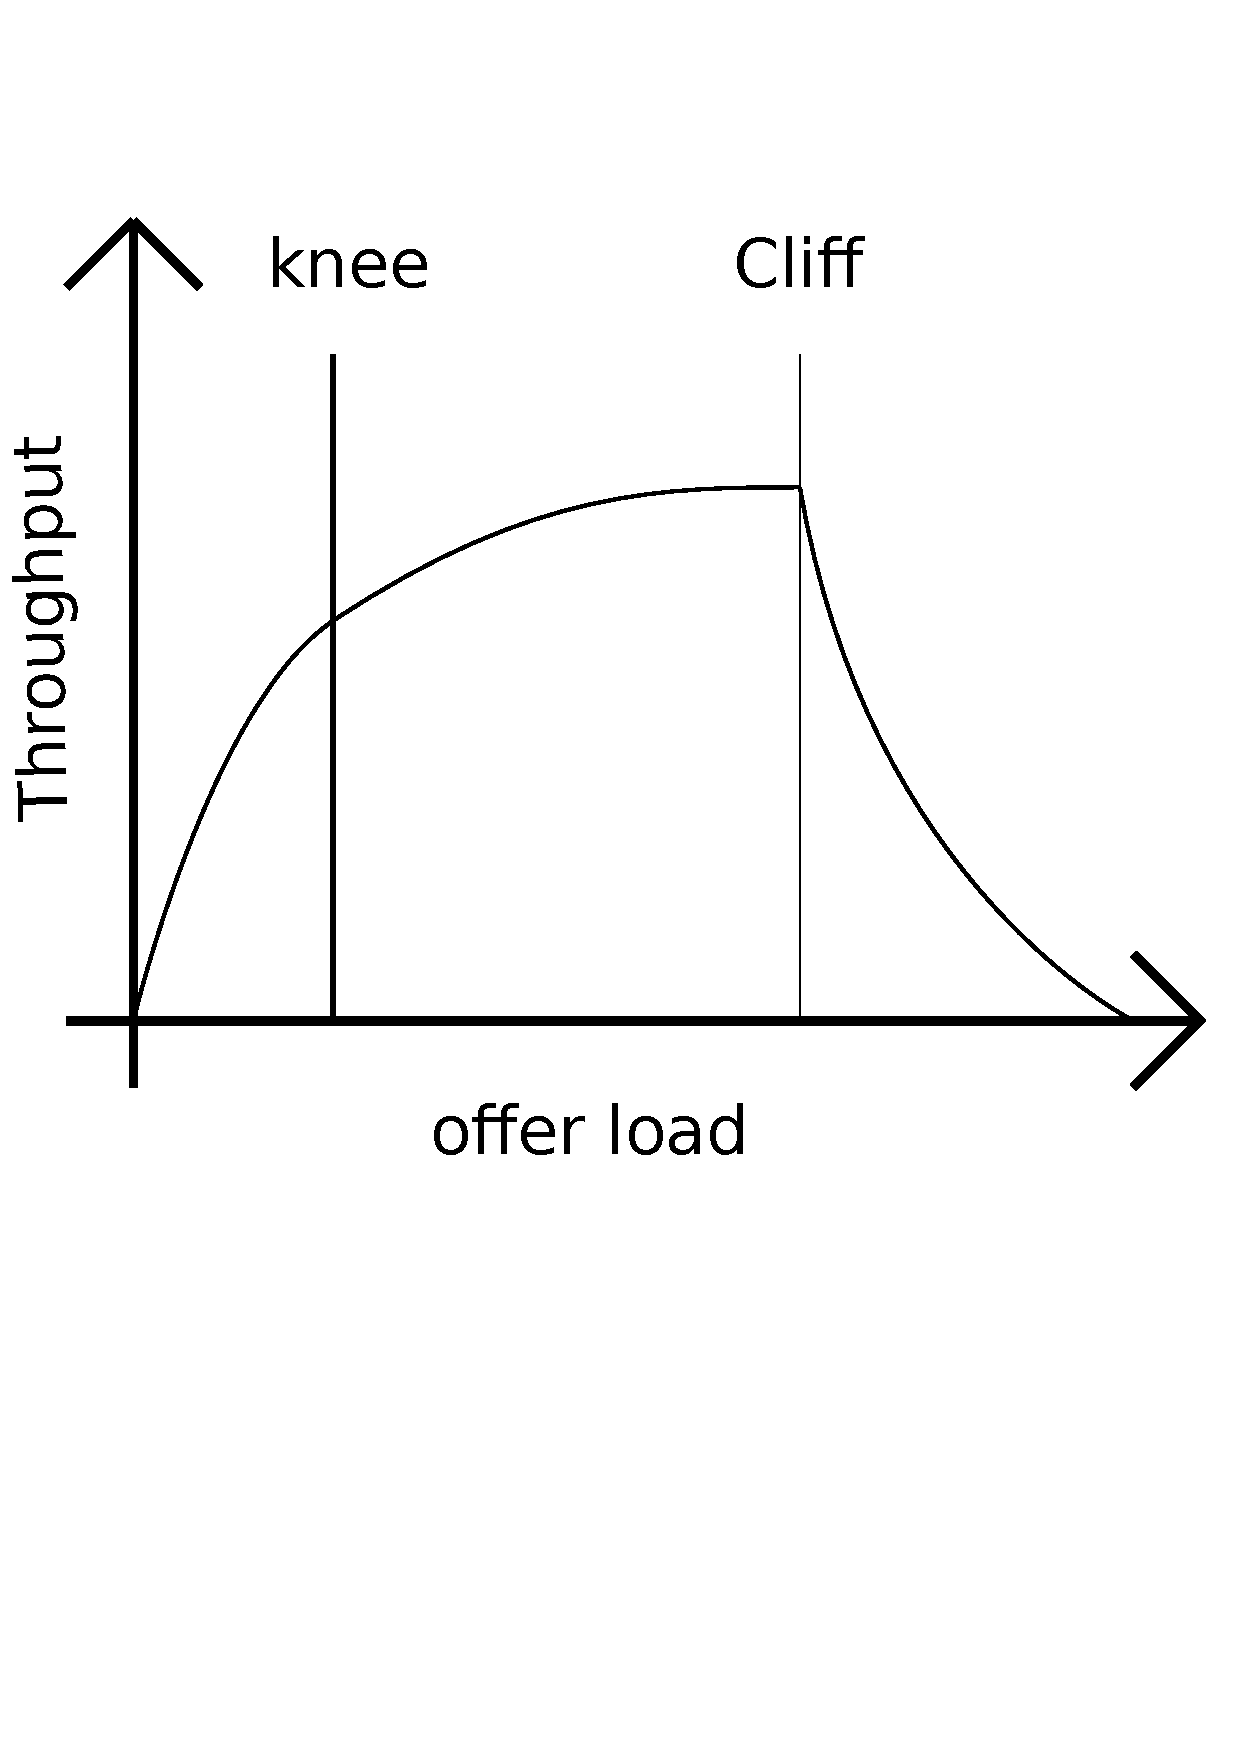
\includegraphics[width=1in]{fig/congestion_throughput} 
  \end{minipage}% 
  \begin{minipage}[t]{0.5\linewidth} 
    \centering  
    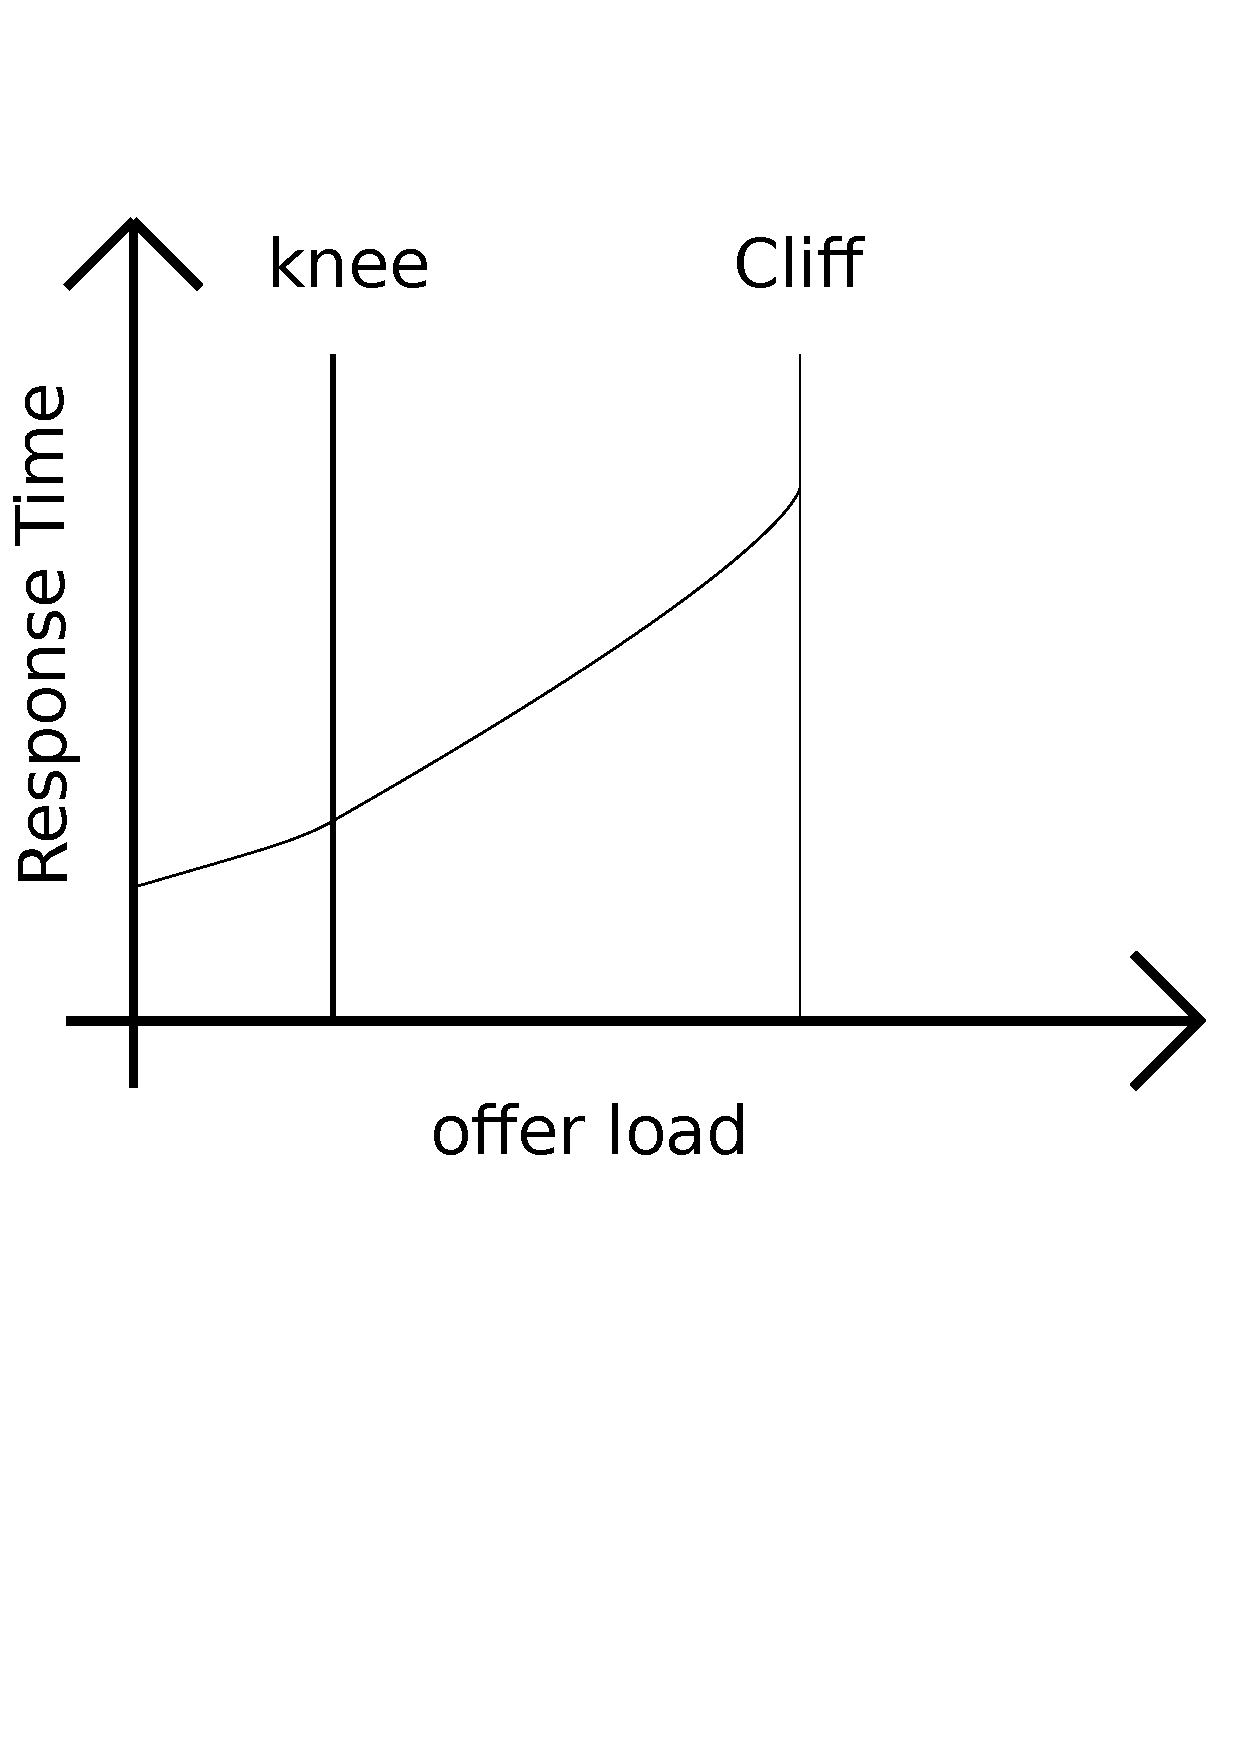
\includegraphics[width=1in]{fig/congestion_ete} 
  \end{minipage} 
  \caption{Congestive collapse}
  \label{fig:problem}
\end{figure}

As figure \ref{fig:problem} shown, when the offer load is low, the throughput of network increases linearly with offer load. The growth of response time is also slow. But when the offer load is higher than knee, the growth of throughput is slow but the response time increase sharply. When the offer load higher than cliff, the throughput fall sharply and response time shard rise. So the object of congestion control is to avoid network enter congestion and take action to clear out
congestion if it occurs. That is said keep the offer load stay between knee and cliff as long as possible.

\subsection{Related studies}

General speaking, there are two paradigms to handle congestion control. One with feedback message and the other without feedback message. For a non-feedback-based mechanism, also known as open-loop control, the edge routers have no information about the state of network and then cannot react to adjust the network offer load. All edge nodes regulate traffic load into network through traffic shaping or traffic rerouting and load balancing based on predefined traffic
description \cite{ref:feedback-based}. The challenge to implement the congestion control by non-feedback-based networks is to pre-determine the traffic parameter, such as average rate and distribution of arrival process at each edge. But also non-feedback-based control scheme can't adjust dynamically. The study of \cite{ref:peak-rate} is a typical open-loop mechanism. Recently, many researchers pay attention to feedback-based network, also refer as close-loop control. There are three stages in feedback-based control, that is detect,feedback,react. The paper \cite{ref:long-term-detect}
compare three detection algorithm. The first based on current traffic information, the second based on single statistic, the third based on multiple statistics. The author conclude that the multiple statistics help improving the estimation accuracy.  
